\subsection{Baseline Controllers}
\label{sec:baseline_comparison}
Both the differential CC and PID baseline controllers were tested on three tasks: following a path, following a trajectory, and repeated the same motion. The results for each are presented in the following sections. The runtime of each controller is presented as well. 

\subsubsection{Path Tracking}
Both baseline controllers were asked to follow five test paths. Each path is discretized into ~50 way points. The controllers are required to measure an end effector position within \SI{2}{cm} of each way point before progressing to the next. The paths traced by each controller is shown in Figures \ref{fig:diff_cc_point_track} and \ref{fig:pid_point_track}. Table \ref{tab:baseline_test_point} highlights key metrics from each run including the total distance travelled by the robot and the time it took to complete each path. This test was repeated three times and the average results across all three trials are displayed. 

\begin{figure}[p]
    \centering
    \makebox[\textwidth][c]{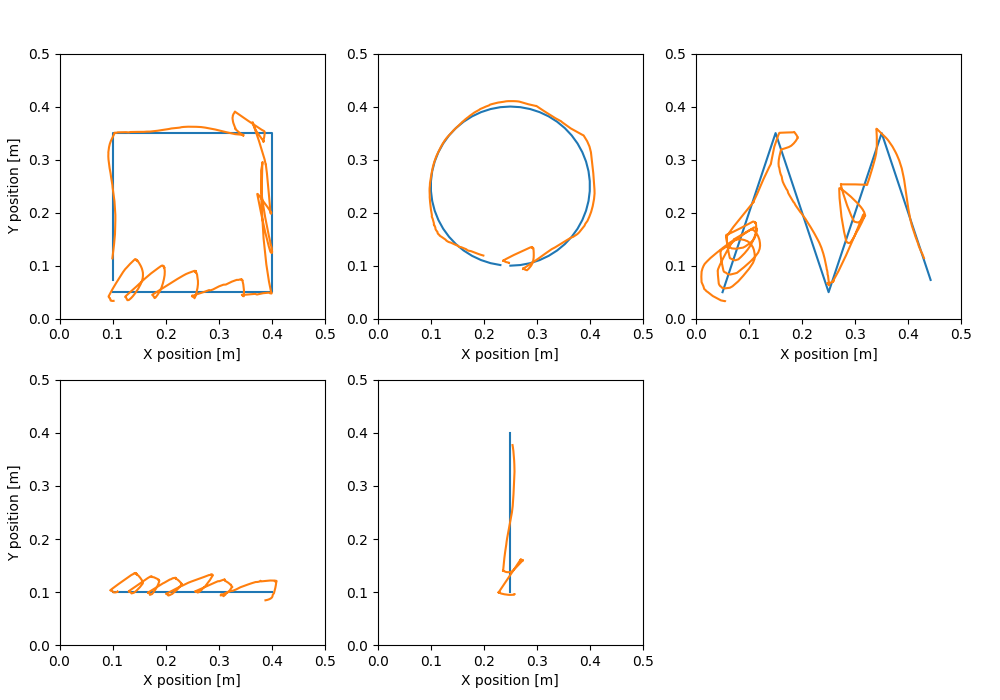
\includegraphics[width=0.95\textwidth]{images/diff_cc_point_tracking.png}}
    \caption{Differential CC controller point tracking path (orange) with reference path (blue) }
    \label{fig:diff_cc_point_track}
\end{figure}

\begin{figure}[p]
    \centering
    \makebox[\textwidth][c]{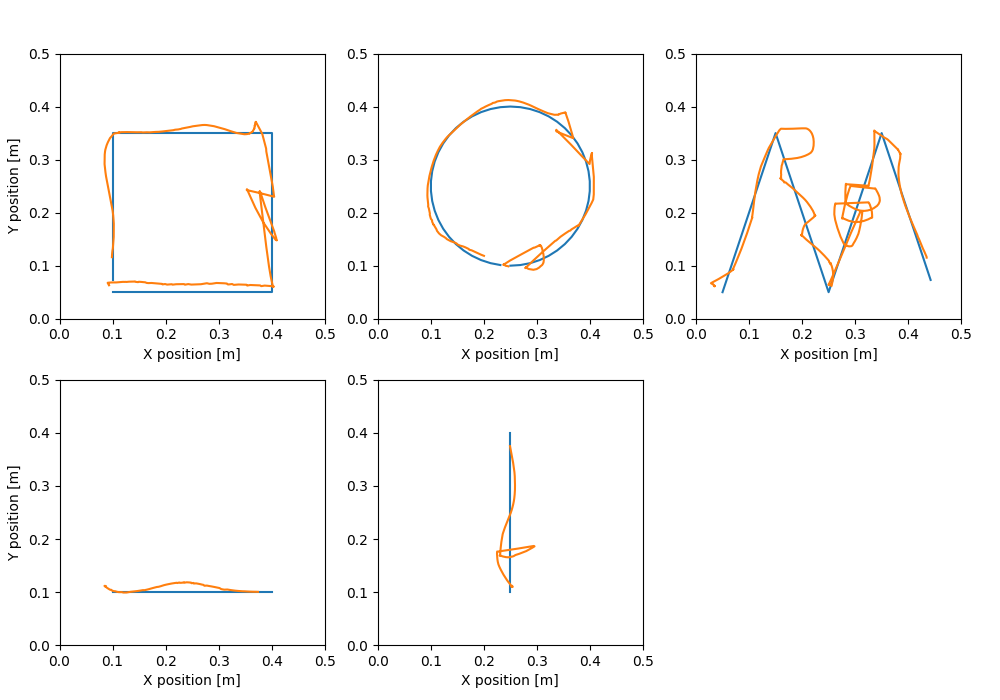
\includegraphics[width=0.95\textwidth]{images/pid_point_tracking.png}}
    \caption{PID controller point tracking path (orange) with reference path (blue)}
    \label{fig:pid_point_track}
\end{figure}

\begin{table}[h]
    \centering
    \caption{Baseline controller point tracking trial summary}
    \begin{tabular}{p{0.27\linewidth} | p{0.17\linewidth} | p{0.2\linewidth} | p{0.2\linewidth}}
        \textbf{Trial Shape} & \textbf{Run time [s]} & \textbf{Path Length [m]} & \textbf{Error}\\
        \hline
        \multicolumn{4}{c}{Reference Trajectory} \\
        \hline
        Square & N/A & 1.178 & N/A \\
        Circle & N/A & 0.923 & N/A \\
        Zig Zag & N/A & 1.241 & N/A \\
        Horizontal Line & N/A & 0.300 & N/A \\
        Vertical Line & N/A & 0.300 & N/A \\
        \hline
        \multicolumn{4}{c}{Differential CC Controller} \\
        \hline
        Square & 136.36 & 2.190 & 85.9\%\\
        Circle & 61.48 & 1.048 & 13.5\%\\
        Zig Zag & 152.21 & 2.551 & 105.6\%\\
        Horizontal Line & 105.48 & 0.817 & 172.3\%\\
        Vertical Line & 34.03 & 0.411& 37.0\%\\
        \hline
        \multicolumn{4}{c}{PID Controller} \\
        \hline
        Square & 74.92 & 1.454 & 23.4\%\\
        Circle & 87.58 & 1.197 & 29.7\%\\
        Zig Zag & 127.87 & 1.988& 60.2\%\\
        Horizontal Line & 19.01 & 0.302 & 0.6\%\\
        Vertical Line & 30.10 & 0.435 & 45\%\\
        \hline
    \end{tabular}   
    \label{tab:baseline_test_point}
\end{table}


\subsubsection{Trajectory Tracking}
Both baseline controllers were asked to execute five test trajectories in a set amount of time. Each trajectory is discretized into ~50 way points with \SI{0.2}{s} in between each. The robot is controlled to follow the way point as it progresses through each of the discretized points. The paths traced by each controller is shown in Figures \ref{fig:diff_cc_traj_track} and \ref{fig:pid_traj_track}. Table \ref{tab:baseline_test_traj} highlights key metrics from each run including the total distance travelled by the robot and the RMSE between the robot path and the test trajectory. 

\begin{figure}[p]
    \centering
    \makebox[\textwidth][c]{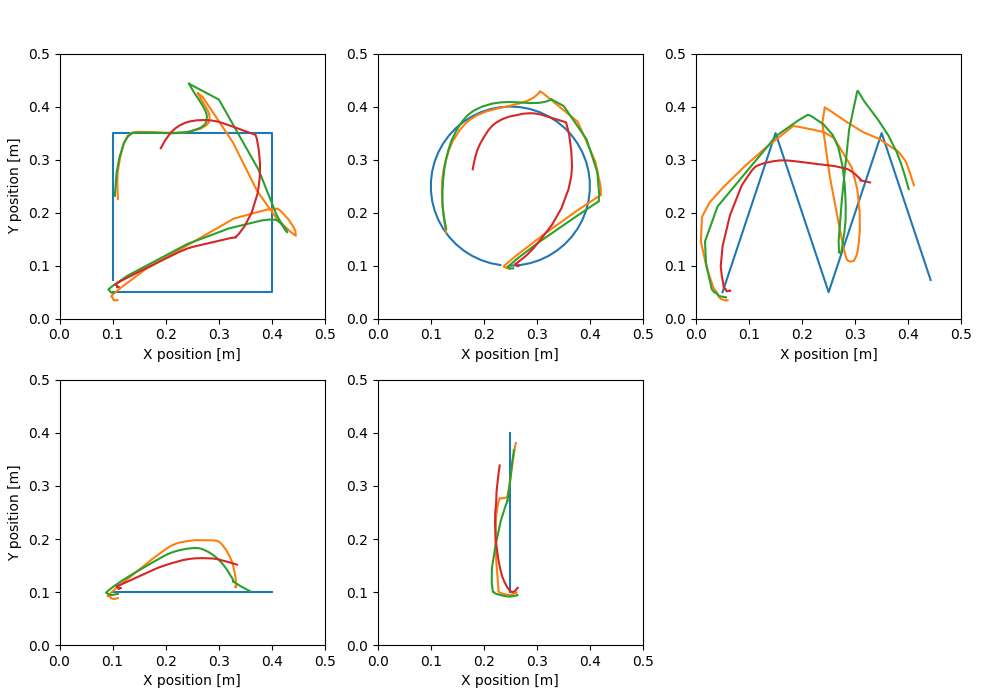
\includegraphics[width=0.95\textwidth]{images/diff_cc_traj_tracking.png}}
    \caption{Differential CC controller trajectory tracking paths (orange, green, red) with reference path (blue)}
    \label{fig:diff_cc_traj_track}
\end{figure}

\begin{figure}[p]
    \centering
    \makebox[\textwidth][c]{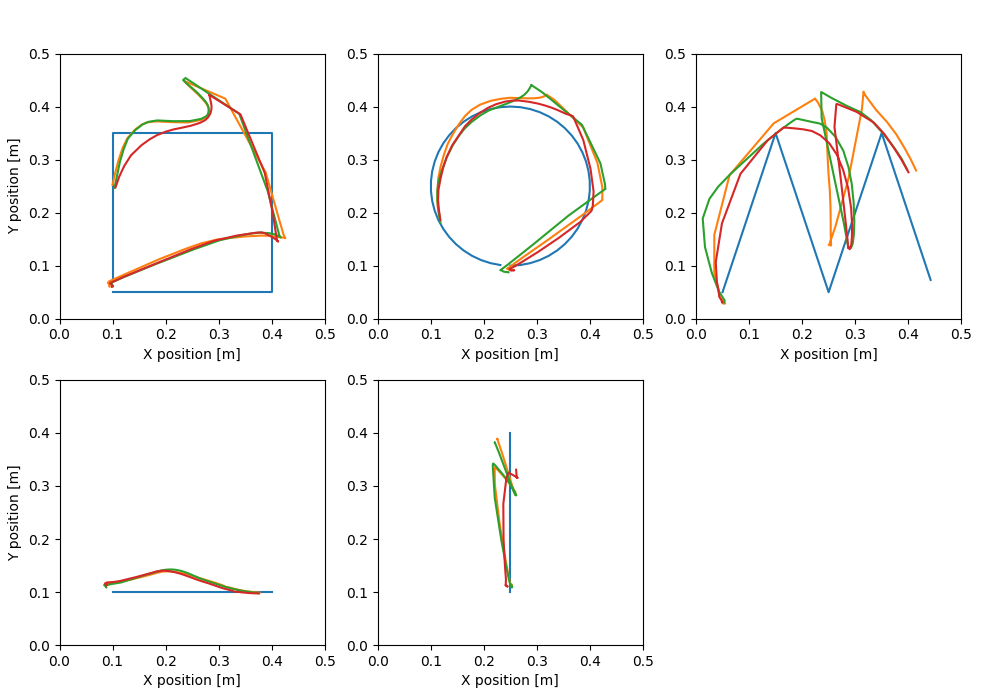
\includegraphics[width=0.95\textwidth]{images/pid_traj_tracking.png}}
    \caption{PID controller trajectory tracking paths (orange, green, red) with reference path (blue)}
    \label{fig:pid_traj_track}
\end{figure}

\begin{table}[h]
    \centering   
    \caption{Baseline controller trajectory tracking trial summary}
    \begin{tabular}{p{0.25\linewidth} | p{0.18\linewidth} | p{0.23\linewidth} | p{0.16\linewidth}}
        \textbf{Trial Shape} & \textbf{Run time [s]} & \textbf{Path Length [m]} & \textbf{RMSE [m]} \\
        \hline
        \multicolumn{4}{c}{Reference Trajectory} \\
        \hline
        Square & 10.80 & 1.178 & N/A\\
        Circle & 10.00 & 0.923 & N/A\\
        Zig Zag & 10.40 & 1.241 & N/A\\
        Horizontal Line & 10.20 & 0.300 & N/A\\
        Vertical Line & 10.20 & 0.300 & N/A\\
        \hline
        \multicolumn{4}{c}{Differential CC Controller} \\
        \hline
        Square & 12.25 & 0.959 & 0.144 \\
        Circle & 11.34 & 0.748 & 0.137 \\
        Zig Zag & 11.80 & 1.008 & 0.147 \\
        Horizontal Line & 11.57 & 0.324 & 0.072 \\
        Vertical Line & 11.57 & 0.305 & 0.055 \\
        \hline
        \multicolumn{4}{c}{PID Controller} \\
        \hline
        Square & 12.22 & 1.031 & 0.131 \\
        Circle & 11.31 & 0.833 & 0.124 \\
        Zig Zag & 11.77 & 11.213 & 0.150 \\
        Horizontal Line & 11.54 & 0.306 & 0.043 \\
        Vertical Line & 11.54 & 0.360 & 0.054 \\
        \hline
    \end{tabular}
    \label{tab:baseline_test_traj}
\end{table}


\subsubsection{Task Repetition}
Controllers were tested on their ability to repeat the same task consistently. The trial was run from home position to the point (\SI{0.15}{m}, \SI{0.2}{m}). It was repeated 10 times for each controller. The paths taken by each controller are shown in Figure \ref{fig:repetition_trial}. The maximal Fréchet distance \cite{frechet_distance} is calculated between each of the 10 trials for both controllers as a metric of controller consistency. The differential CC controller has a maximal Fréchet distance of \SI{0.102}{m} while the PID controller has a maximal Fréchet distance of \SI{0.027}{m}, indicating a much tighter distribution. This result is confirmed visually in Figure \ref{fig:repetition_trial}. 

\begin{figure}[h]
     \centering
     \begin{subfigure}[b]{0.48\textwidth}
         \centering
         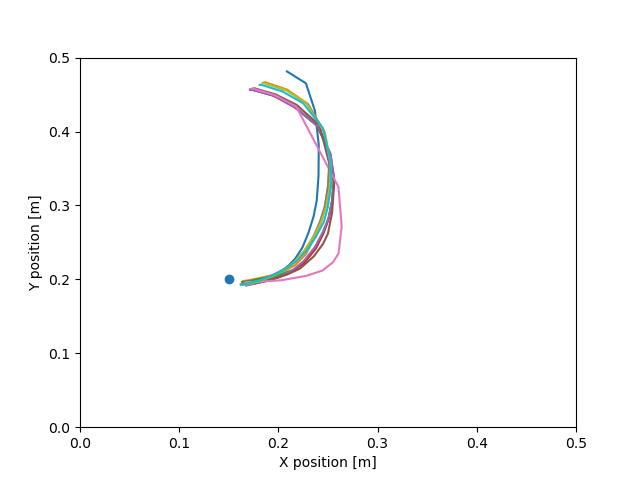
\includegraphics[width=\textwidth]{images/diff_cc_repetition.png}
         \caption{Differential CC controller task repetition}
         \label{fig:diff_cc_repetition}
     \end{subfigure}
     \hfill
     \begin{subfigure}[b]{0.48\textwidth}
         \centering
         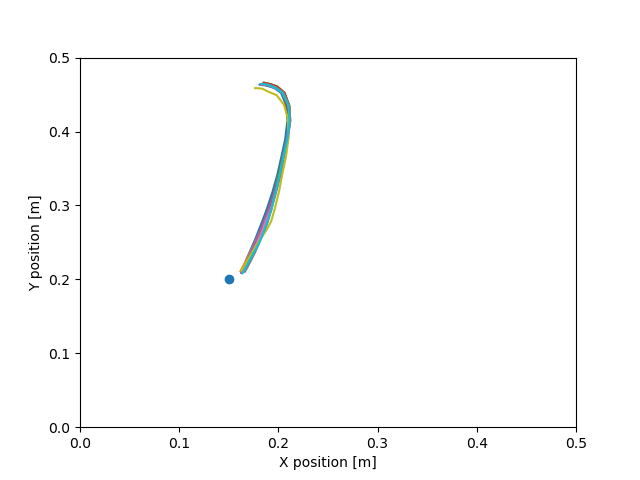
\includegraphics[width=\textwidth]{images/pid_repetition.png}
         \caption{PID controller task repetition}
         \label{fig:pid_repetition}
     \end{subfigure}
        \caption{Baseline controller repeated motion trial paths. The target point is shown in blue.}
        \label{fig:repetition_trial}
\end{figure}


\subsubsection{Timing Analysis}
The runtime of four different necessary controller functions was studied for both baseline controllers and the best performing learned controller. This includes the controller constructor method, the command retrieval, the end point update, and the goal point update. Table \ref{tab:runtimes} displays the results. A "per iteration" result is returned as well, which is a sum of the three functions that are required to run at each control loop. 

\begin{table}[h]
    \centering   
    \caption{Controller run times}
    \begin{tabular}{p{0.4\linewidth} | p{0.2\linewidth} }
        \textbf{Function} & \textbf{Run time [$\mu$s]} \\
        \hline
        \multicolumn{2}{c}{Differential CC Controller} \\
        \hline
        Current command retrieval & 0.1 \\
        End point update & 364.2 \\
        Goal point update & 0.2 \\
        \textbf{Total per iteration} & \textbf{364.5} \\
        Controller object construction & 11.4 \\
        \hline
        \multicolumn{2}{c}{PID Controller} \\
        \hline
        Current command retrieval & 0.1 \\
        End point update & 24.5 \\
        Goal point update & 0.8 \\
        \textbf{Total per iteration} & \textbf{25.4} \\
        Controller object construction & 211.0 \\
        \hline
        \multicolumn{2}{c}{Learning-Based Controller} \\
        \hline
        Current command retrieval & 0.2 \\
        End point update & 356.3 \\
        Goal point update & 0.2 \\
        \textbf{Total per iteration} & \textbf{356.7} \\
        Controller object construction & 1,184.3 \\
        \hline
    \end{tabular}
    \label{tab:runtimes}
\end{table}

